\documentclass[12pt]{article}
\usepackage{amsfonts, amssymb, amsmath, amsthm}
\usepackage[margin=1in]{geometry}
\usepackage{tikz}
\usetikzlibrary{patterns, decorations.pathreplacing, arrows.meta}

\pagestyle{myheadings}
\markright{Explainer: Rudin 1.9 — Lexicographic Order on $\mathbb{C}$\hfill}

\newcommand{\R}{\mathbb{R}}
\newcommand{\Q}{\mathbb{Q}}
\newcommand{\C}{\mathbb{C}}

\begin{document}

\begin{center}
    \textbf{\Large Lexicographic Order on $\mathbb{C}$}\\[0.5em]
    \large A visual guide to Rudin 1.9
\end{center}

\section{What is Lexicographic Order?}

``Lexicographic'' means ``dictionary order.'' Compare the first component; if equal, compare the second.

For $z = a + bi$ and $w = c + di$:
\[
z < w \quad \Longleftrightarrow \quad (a < c) \text{ or } (a = c \text{ and } b < d)
\]

\section{Visual: How the Order Works}

\begin{center}
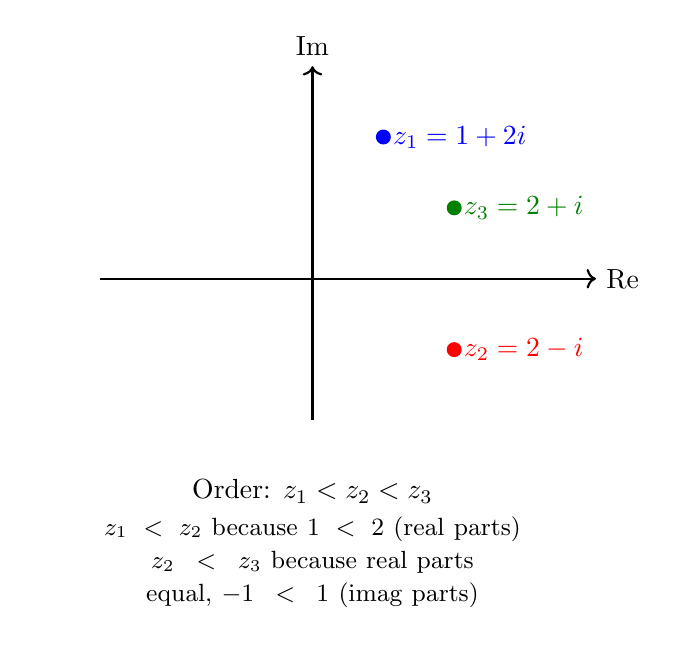
\begin{tikzpicture}[scale=0.9]
    % Axes
    \draw[thick, ->] (-3, 0) -- (4, 0) node[right] {Re};
    \draw[thick, ->] (0, -2) -- (0, 3) node[above] {Im};

    % Points
    \fill[blue] (1, 2) circle (3pt) node[right] {$z_1 = 1 + 2i$};
    \fill[red] (2, -1) circle (3pt) node[right] {$z_2 = 2 - i$};
    \fill[green!50!black] (2, 1) circle (3pt) node[right] {$z_3 = 2 + i$};

    % Ordering
    \node at (0, -3) {Order: $z_1 < z_2 < z_3$};
    \node[text width=7cm, align=center] at (0, -4) {\small $z_1 < z_2$ because $1 < 2$ (real parts)\\
    $z_2 < z_3$ because real parts equal, $-1 < 1$ (imag parts)};
\end{tikzpicture}
\end{center}

\section{The ``Dictionary'' Analogy}

\begin{center}
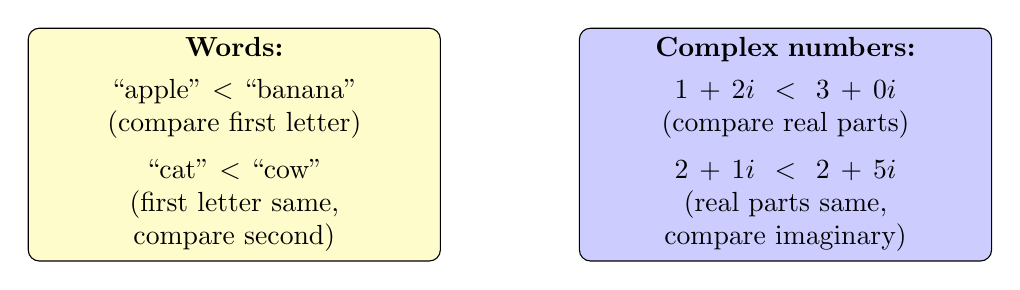
\begin{tikzpicture}
    \node[draw, rounded corners, fill=yellow!20, text width=5cm, align=center] at (-3.5, 0) {
        \textbf{Words:}\\[0.3em]
        ``apple'' $<$ ``banana''\\
        (compare first letter)\\[0.5em]
        ``cat'' $<$ ``cow''\\
        (first letter same,\\compare second)
    };

    \node[draw, rounded corners, fill=blue!20, text width=5cm, align=center] at (3.5, 0) {
        \textbf{Complex numbers:}\\[0.3em]
        $1 + 2i < 3 + 0i$\\
        (compare real parts)\\[0.5em]
        $2 + 1i < 2 + 5i$\\
        (real parts same,\\compare imaginary)
    };
\end{tikzpicture}
\end{center}

\section{Is This a Total Order?}

We need to verify four properties:

\subsection{Reflexive: $z \leq z$}
Trivially true since $z = z$.

\subsection{Anti-symmetric: $z \leq w$ and $w \leq z$ implies $z = w$}

\begin{center}
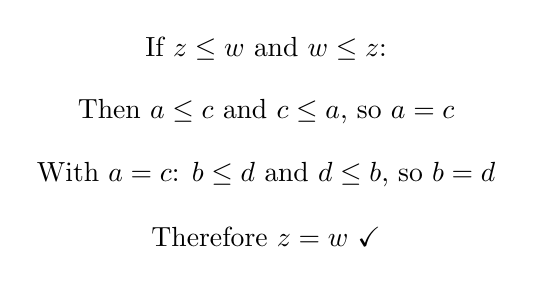
\begin{tikzpicture}[scale=0.8]
    \node at (0, 1) {If $z \leq w$ and $w \leq z$:};
    \node at (0, 0) {Then $a \leq c$ and $c \leq a$, so $a = c$};
    \node at (0, -1) {With $a = c$: $b \leq d$ and $d \leq b$, so $b = d$};
    \node at (0, -2) {Therefore $z = w$ \checkmark};
\end{tikzpicture}
\end{center}

\subsection{Transitive: $z \leq w$ and $w \leq u$ implies $z \leq u$}

\begin{center}
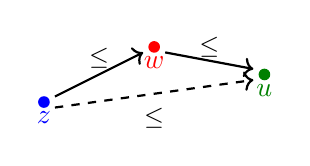
\begin{tikzpicture}[scale=0.7]
    \fill[blue] (0, 0) circle (3pt) node[below] {$z$};
    \fill[red] (2, 1) circle (3pt) node[below] {$w$};
    \fill[green!50!black] (4, 0.5) circle (3pt) node[below] {$u$};

    \draw[->, thick] (0.2, 0.1) -- (1.8, 0.9);
    \draw[->, thick] (2.2, 0.9) -- (3.8, 0.6);
    \draw[->, thick, dashed] (0.2, -0.1) -- (3.8, 0.4);

    \node at (1, 0.8) {\small $\leq$};
    \node at (3, 1) {\small $\leq$};
    \node at (2, -0.3) {\small $\leq$};
\end{tikzpicture}
\end{center}

\subsection{Comparable: For any $z, w$, either $z \leq w$ or $w \leq z$}

Since $\mathbb{R}$ is totally ordered, we can always compare $a$ with $c$:
\begin{itemize}
    \item If $a < c$: then $z < w$
    \item If $a > c$: then $w < z$
    \item If $a = c$: compare $b$ with $d$ (same logic)
\end{itemize}

\section{Does It Have the Least Upper Bound Property?}

\textbf{NO!}

\subsection{The Counterexample}

Consider $A = \{z = a + bi : a < 1\}$ (everything to the left of the line $\text{Re}(z) = 1$).

\begin{center}
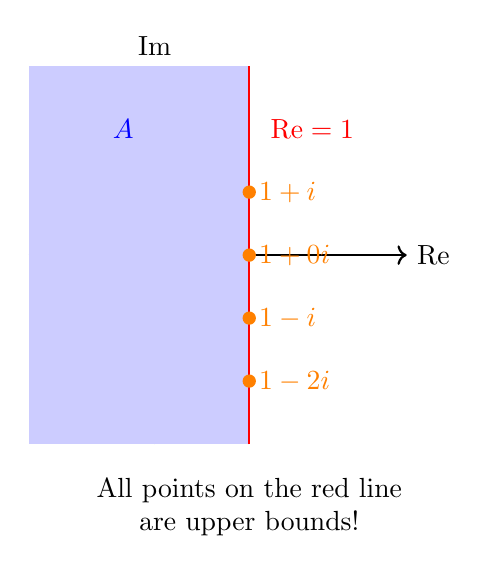
\begin{tikzpicture}[scale=0.8]
    % Axes
    \draw[thick, ->] (-2, 0) -- (4, 0) node[right] {Re};
    \draw[thick, ->] (0, -3) -- (0, 3) node[above] {Im};

    % The set A (shaded region)
    \fill[blue!20] (-2, -3) rectangle (1.5, 3);
    \draw[blue, thick, dashed] (1.5, -3) -- (1.5, 3);
    \node[blue] at (-0.5, 2) {$A$};

    % The line Re = 1
    \draw[red, thick] (1.5, -3) -- (1.5, 3);
    \node[red] at (2.5, 2) {$\text{Re} = 1$};

    % Upper bounds
    \fill[orange] (1.5, 1) circle (3pt) node[right] {$1 + i$};
    \fill[orange] (1.5, 0) circle (3pt) node[right] {$1 + 0i$};
    \fill[orange] (1.5, -1) circle (3pt) node[right] {$1 - i$};
    \fill[orange] (1.5, -2) circle (3pt) node[right] {$1 - 2i$};

    \node[text width=5cm, align=center] at (1.5, -4) {All points on the red line\\are upper bounds!};
\end{tikzpicture}
\end{center}

\subsection{Why No Least Upper Bound?}

Upper bounds of $A$ are points with real part $\geq 1$.

Among those with real part exactly $1$: $\{1 + bi : b \in \mathbb{R}\}$

\begin{center}
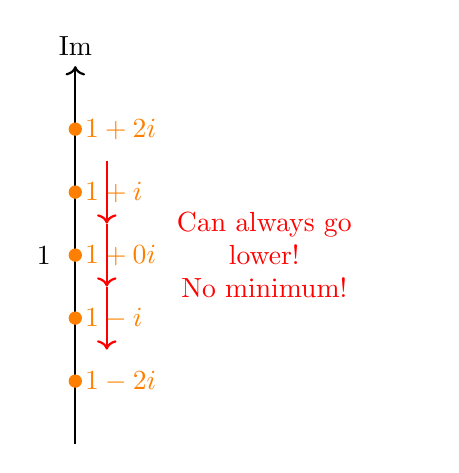
\begin{tikzpicture}[scale=0.8]
    \draw[thick, ->] (0, -3) -- (0, 3) node[above] {Im};
    \node at (-0.5, 0) {$1$};

    \fill[orange] (0, 2) circle (3pt) node[right] {$1 + 2i$};
    \fill[orange] (0, 1) circle (3pt) node[right] {$1 + i$};
    \fill[orange] (0, 0) circle (3pt) node[right] {$1 + 0i$};
    \fill[orange] (0, -1) circle (3pt) node[right] {$1 - i$};
    \fill[orange] (0, -2) circle (3pt) node[right] {$1 - 2i$};

    \draw[->, thick, red] (0.5, 1.5) -- (0.5, 0.5);
    \draw[->, thick, red] (0.5, 0.5) -- (0.5, -0.5);
    \draw[->, thick, red] (0.5, -0.5) -- (0.5, -1.5);

    \node[red, text width=4cm, align=center] at (3, 0) {Can always go\\lower!\\No minimum!};
\end{tikzpicture}
\end{center}

For any candidate $1 + ci$, we have $1 + (c-1)i < 1 + ci$, and $1 + (c-1)i$ is still an upper bound.

So there's no \textbf{least} upper bound!

\section{Summary}

\begin{center}
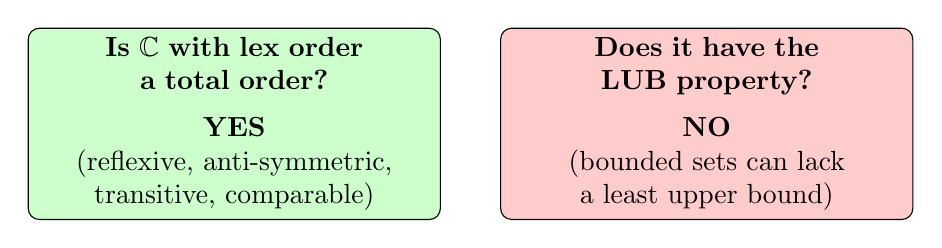
\begin{tikzpicture}
    \node[draw, rounded corners, fill=green!20, text width=5cm, align=center] at (-3, 0) {
        \textbf{Is $\mathbb{C}$ with lex order\\a total order?}\\[0.5em]
        \textbf{YES}\\
        (reflexive, anti-symmetric,\\transitive, comparable)
    };

    \node[draw, rounded corners, fill=red!20, text width=5cm, align=center] at (3, 0) {
        \textbf{Does it have the\\LUB property?}\\[0.5em]
        \textbf{NO}\\
        (bounded sets can lack\\a least upper bound)
    };
\end{tikzpicture}
\end{center}

\end{document}
